\documentclass[twoside,11pt]{article}
\usepackage{amssymb,amsmath, amsfonts,latexsym,mathtext, array, graphicx, geometry, caption, subcaption}
\geometry{margin=1.5cm}
\setlength{\parskip}{0.8ex plus 0.1ex minus 0.2ex}
\newcommand{\M}[1]{\boldsymbol{\mathbf{#1}}}
\newcommand{\V}{\M}
\newcommand{\Cal}{\mathcal}

\newtheorem{thm1}{Theorem}
\newtheorem{def1}{Definition}

\begin{document}

\title{Machine Learning 6.867 - Project}

\maketitle
%!TEX root = paper.tex

\section{Introduction}\label{sec:intro}
%!TEX root = paper.tex

\section{Mean-Field Variational Bayes}\label{sec:mfvb}

Mean-field variational Bayes (MFVB) is a method for approximating the posterior distribution.  In general, we have unknown parameters $w_1, w_2, \ldots, w_n$ that we have priors on, and our objective is to find the joint distribution $p(w_1, w_2, \ldots, w_n)$.  Assuming that our approximate distribution is in the family $Q = \{q : q(w_1, w_2, \ldots, w_n) = q(w_1)q(w_2) \ldots q(w_n)\}$, we find $q^* \in Q$ that minimizes the KL-divergence with $p$, i.e. $q^* = \min KL(q || p)$. 
In particular, for logistic regression, the analytical form of the posterior is unknown and has been approximated with MFVB in the literature [2]. We use local variational bounds on the conditional probability using the convexity of the logarithm function. In particular, we use a variational treatment based on the approach of Jaakkola and Jordan (2000). 
This approach consists of approximation the likelihood function of the logistic regression, governed by the sigmoid function, by the exponential of the a quadratic form, leading to a gaussian approximation of the posterior distribution. More explicitly, if $y\in \{-1,1\}$ is a target variable for a data vector $x$ then the likelihood function of the target variable $y$ is: 
\begin{equation}
p(y | x, w)=\sigma(y w^T x)
\end{equation}

with $w$ being the logistic regression weight, and $\sigma(x)=\dfrac{1}{1+\exp(-x)}$ the sigmoid function. 
Using a transformation of a the logarithm of the sigmoid and the concept of convex duality, we get: 
\begin{equation}
\sigma(x) \geq \sigma(\xi)\exp((x-\xi)/2-\lambda(\xi)(x^2-\xi^2))
\end{equation}

where
$$\lambda(\xi)=\frac{1}{2\xi}[\sigma(\xi)-\frac{1}{2}]=\frac{1}{4\xi}\tanh(\frac{\xi}{2})$$
and $\xi$ is a variational parameter. 

Therefore, if we let $a=w^T x$ we get: 
\begin{equation}
p( y | x,w)\geq e^{ya} \sigma(\xi)\exp\{-(\xi+a)/2-\lambda(\xi)(a^2-\xi^2)\}
\end{equation}

To every training set observation $(x_n, y_n)$, there is a variational parameter $\xi_n$ associated. We apply the bound above to each of the terms in the likelihood function. Let $Y=[y_1, y_2, \ldots , y_n]^T$ and the $X$ be the data matrix, then the likelihood function is: 
\begin{equation}
p( Y | X, w)=\prod_{i=1}^{N} p(y_i | x_i, w) = \prod_{i=1}^{N} \sigma(y w^T x)
\end{equation}

and thus we obtain the following bound on the marginal data likelihood :
\begin{equation}
p( Y | X, w) \geq h(w, \xi)
\end{equation}
and 
$$h(w,\xi) = \prod_{i=1}^{N} e^{y_iw^T x_i} \sigma(\xi_i)\exp\{-(\xi_i+w^T x_i)/2-\lambda(\xi_i)((w^T x_i)^2-{\xi_i}^2)\}$$

This approximation is used because the sigmoid data likelihood does not have a conjugate in the exponential family of priors. The approximation we yielded is quadratic in $w$ in the exponential, and we use the conjugate gaussian prior :
\begin{equation}
p( w | \alpha) = \mathcal{N}(0, \alpha ^{-1} \mathcal{I})
\end{equation}
and we can also model the hyper-parameter $\alpha$ with a conjugate Gamma distribution : 
\begin{equation}
p(\alpha) = Gam( \alpha | a_0, b_0)
\end{equation}

Variational Bayesian inference aims at maximizing a lower bound of the data log-likelihood. The log-likelihood is
\begin{equation}
\ln p(Y| X)=\ln \int\int p(Y| X, w) p(w |\alpha)p(\alpha)dw d\alpha
\end{equation}

We approximate the posterior $p(w, \alpha | X)$ by the variational distribution $Q(w, \alpha)$ that can be factorized to $Q(\alpha)Q(w)$. The bound of the log-likelihood is as follows : 
\begin{equation}
\ln p(Y| X) \geq \mathcal{L}(Q)=\ln \int\int Q(w, \alpha) \ln \dfrac{p(Y| X, w) p(w |\alpha)p(\alpha)}{Q(w,\alpha)}dw d\alpha
\end{equation}

Hence, using Equation (5), obtain a variational bound $ \mathcal{\tilde{L}}(Q, \xi) $  that we aim at maximizing:
\begin{equation}
\mathcal{\tilde{L}}(Q, \xi)=\int\int Q(w, \alpha) \ln \dfrac{h(w,\xi) p(w |\alpha)p(\alpha)}{Q(w,\alpha)}dw d\alpha
\end{equation}

After we substitute $Q(w, \alpha)$ with $Q(\alpha)Q(w)$ and we calculate the expectations of 
$alpha$ and $w$ as in the general MFVB, we obtain this expression of  $ \mathcal{\tilde{L}}(Q, \xi) $: 
\begin{equation}
\mathcal{\tilde{L}}(Q, \xi)=\frac{1}{2}w_N^T V_N^{-1} w_N + \frac{1}{2} \ln |V_N| + \sum_{n} \left( \ln \sigma(\xi_n) - \frac{\xi_n}{2} + \lambda(\xi_n)\xi_n^2\right)-\ln \Gamma(a_0) +a_0 \ln(b_0)-b_0\frac{a_N}{b_N}-a_N \ln(b_N)-\ln \Gamma(a_N) +a_N
\end{equation}
with 
$$a_N=a_0 +\frac{D}{2} $$
$$b_N=b_0+\frac{1}{2}w_N^T w_N +Tr(V_N)$$
$$V_N^{-1}=\frac{a_N}{b_N} \mathcal{I} +2 \sum_{n} \lambda(\xi_n)x_n x_n^T$$
$$w_N=V_N \sum_{n}\frac{y_n}{2}x_n $$

and 
$$Q ^ *(w)=\mathcal{N}(w | w_N, V_N)$$ 
$$Q^ *(\alpha)=Gam(\alpha | a_N, b_N)$$
This bound depends on $\xi$. We maximize this bound with respect to $\xi$ and we find : 
\begin{equation}
(\xi_n^{new})^2=x_n^T (V_N +w_Nw_N ^T) x_N
\end{equation}


We use the EM algorithm to update the equations for $ w_N , V_N, a_N, b_N, \text{and}  \xi $ in order to maximize the variational bound $\mathcal{\tilde{L}}(Q, \xi)$ , until it reaches a plateau. 



%!TEX root = paper.tex

\section{Markov-Chain Monte Carlo}\label{sec:mcmc}

To evaluate the quality of the covariance estimates produced by our method, we used Markov-Chain Monte Carlo (MCMC) as a benchmark for the ``true'' distribution of the logistic regression weights $(w_0, w_1, w_2)$.  We used the \texttt{R} package \texttt{MCMCpack} with an improper uniform prior, 10,000 iterations, and burn-in rate of 1,000 iterations.  We also compared to
an MCMC simulation with a normal prior on the weights $\mathcal{N}(\M{0},1000I)$ and found similar results. Figures~\ref{fig:mcmc_iterations} and \ref{fig:mcmc_iterations_normal} show the progression of the MCMC algorithm assuming each prior.  

\begin{figure}
\centering
	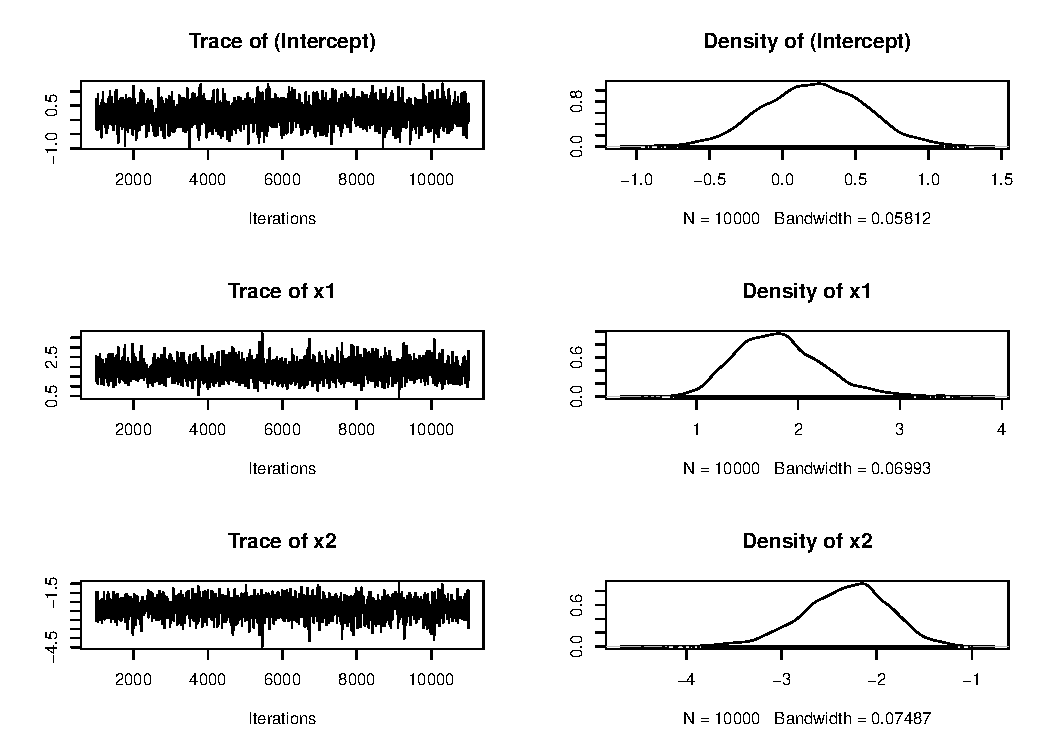
\includegraphics[height=100mm]{figures/mcmc_uniform.pdf}
    \caption{MCMC simulations of logistic regression weights for dataset 1, and corresponding marginal density plots, assuming 
    an improper uniform prior. 10,000 iterations total.}  \label{fig:mcmc_iterations}  
\end{figure}

\begin{figure}
\centering
	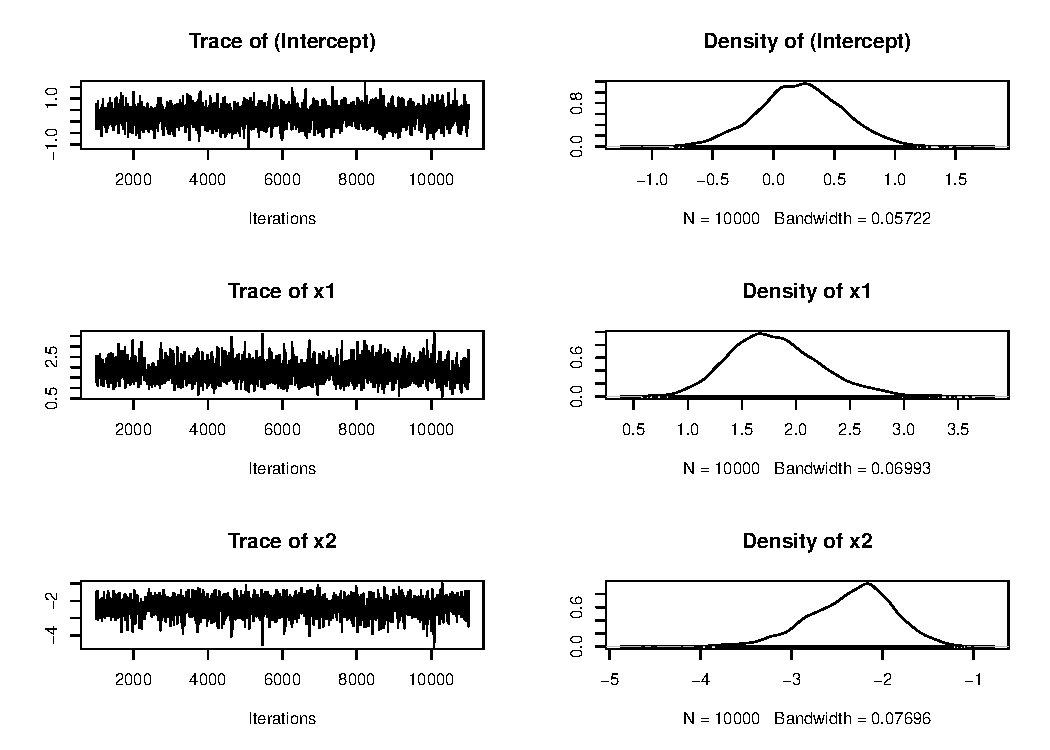
\includegraphics[height=100mm]{figures/mcmc_normal.pdf}
    \caption{MCMC simulations of logistic regression weights for dataset 1, and corresponding marginal density plots, assuming 
    a normal prior $\mathcal{N}(\M{0},1000I)$. 10,000 iterations total.}  \label{fig:mcmc_iterations_normal}  
\end{figure}

To visualize the joint distribution of the logistic regression weights, we plot the MCMC results for the values of $w_1$ and $w_2$.  In addition, we fit the kernel density to the 

\begin{table}[tb]
\centering
\begin{tabular}{rcccccc}
  \toprule
 {\bf  Dataset} & {\bf  Logit Train} & {\bf  Logit Test} & {\bf  MCMC Train} & {\bf  MCMC Test} & {\bf  MFVB Train} & {\bf  MFVB Test}\\
  \midrule
  0 & 0.8700 & {\bf 0.8580} & 0.8700 & {\bf 0.8580} & 0.8600 & 0.8570 \\
  1 & 0.7500 & 0.8450 & 0.7500 & {\bf 0.8460} & 0.7400 & 0.8450 \\
  2 & 0.5500 & {\bf 0.4890} & 0.5100 & {\bf 0.4890} & 0.5400 & 0.4750 \\
  3 & 0.6900 & {\bf 0.7420} & 0.6900 & {\bf 0.7420} & 0.7200 & 0.7120 \\
  4 & 0.8600 & {\bf 0.8050} & 0.8600 & {\bf 0.8050} & 0.8600 & 0.8040 \\
  5 & 0.9400 & 0.9290 & 0.9400 & {\bf 0.9300} & 0.9400 & 0.9260 \\
  6 & 0.7400 & 0.7130 & 0.7400 & {\bf 0.7140} & 0.6900 & 0.6840 \\
  7 & 1.0000 & 0.9760 & 1.0000 & *** & 1.0000 & {\bf 0.9780} \\
  8 & 0.9200 & {\bf 0.8670} & 0.9200 & {\bf 0.8670} & 0.9300 & 0.8640 \\
  9 & 0.5200 & 0.3980 & 0.5100 & 0.4020 & 0.4600 & {\bf 0.4130} \\
  10 & 0.6700 & 0.6690 & 0.6700 & {\bf 0.6700} & 0.6300 & 0.6560 \\
  \bottomrule
\end{tabular}
\caption{Training and test set accuracy for logistic regression, MCMC logistic regression, and MFVB logistic regression on all datasets.  The highest out-of-sample accuracy score is highlighted for each dataset.  \\ *** : The training dataset was completely separable; therefore the posterior covariance matrix was zero and the precision matrix was undefined.  Thus, we did not obtain MCMC predictive probabilities for this dataset. }\label{tab:all_acc}
\end{table}


\begin{figure}
\centering
	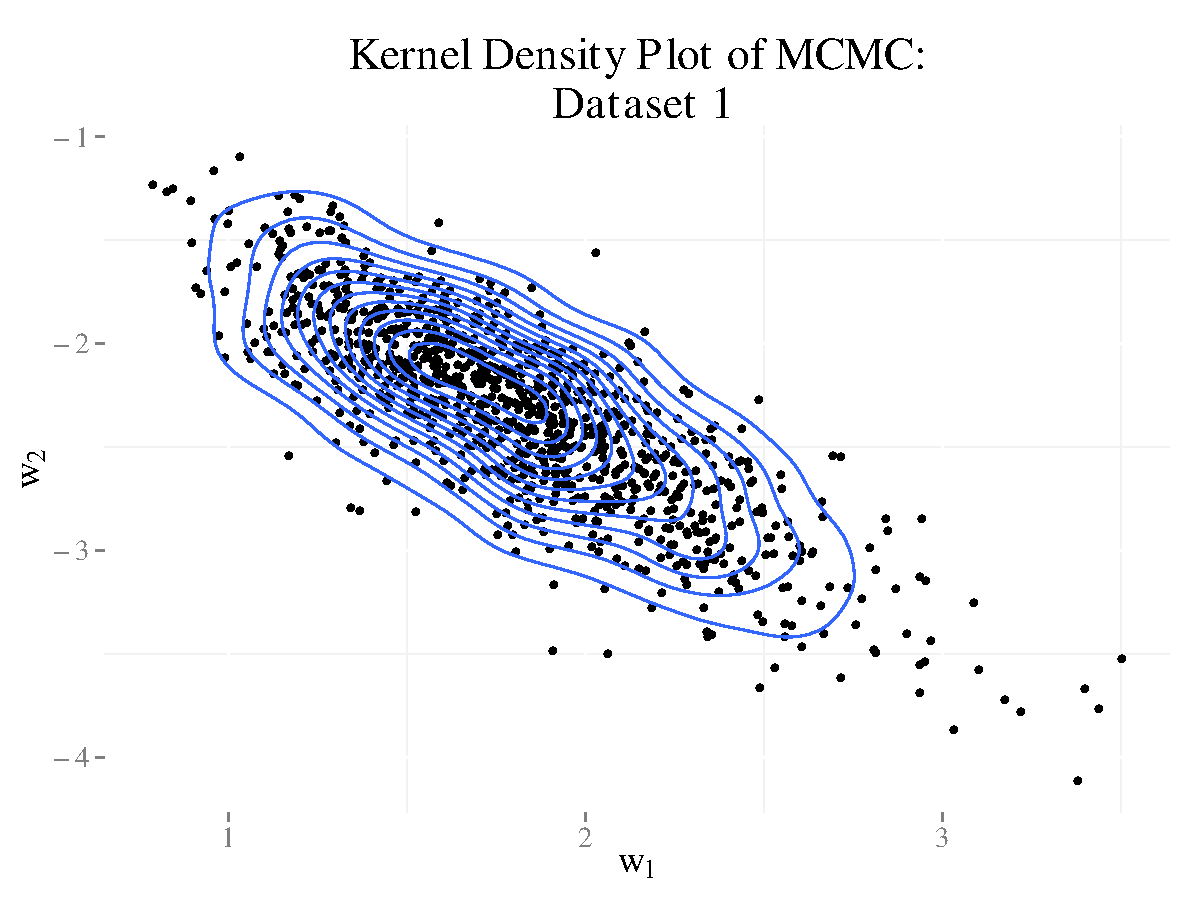
\includegraphics[height=120mm]{figures/mcmc_uniform_2d.pdf}
    \caption{MCMC simulations of logistic regression weights for dataset 1, and corresponding kernel density plot, assuming 
    an improper uniform prior.  Subset of 1,000 out of 10,000 total iterations shown.}  \label{fig:mcmc_kernel}  
\end{figure}

\begin{figure}
\centering
	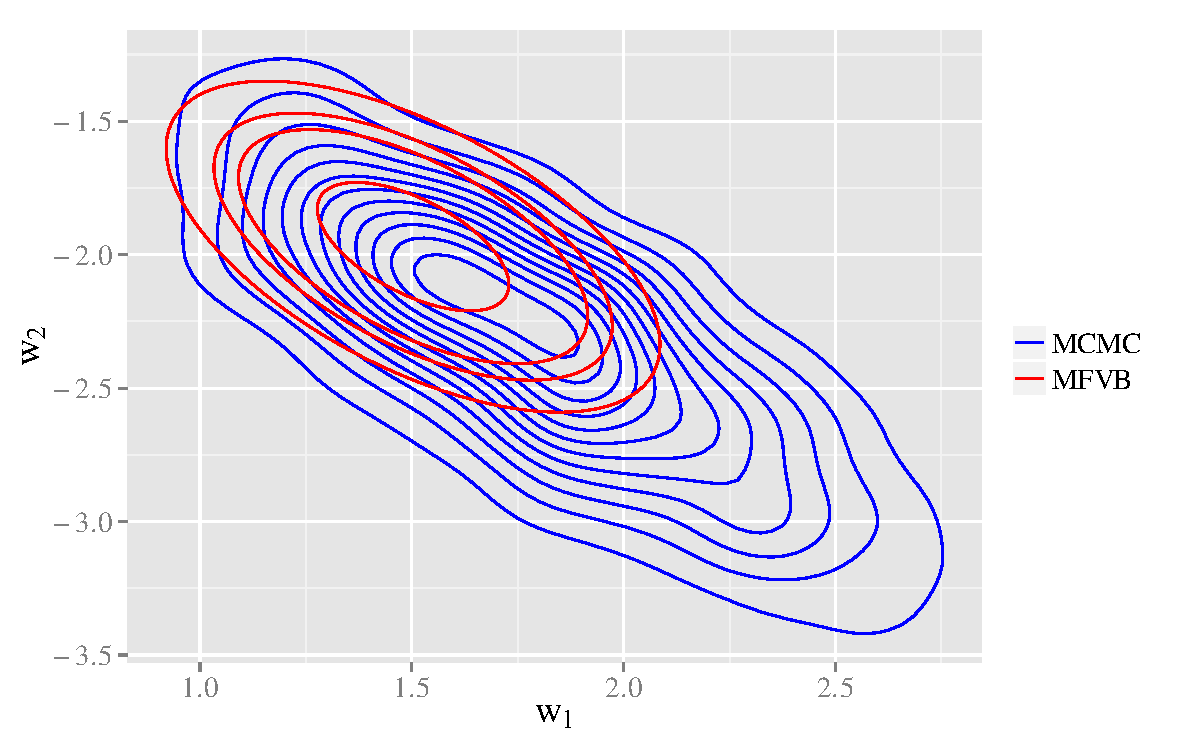
\includegraphics[height=120mm]{figures/mcmc_uniform_mfvb.pdf}
    \caption{Comparison of logistic regression point estimate, kernel density plot of MCMC simulations, and posterior density of
    MFVB logistic regression (vectorized function), for dataset 1.   Contours of MFVB logistic regression indicate
    50\%, 90\%, 95\%, and 99\% confidence intervals for the bivariate normal $\mathcal{N}(\M{w}_{N},\M{V}_N)$.
    Mean values for MCMC and MFVB are also included.}  \label{fig:mcmc_mfvb}  
\end{figure}

\end{document}